% !TeX root = RJwrapper.tex
\title{nlmeVPC: Visual Model Diagnosis for the Nonlinear Mixed Effect Model}
\author{by Eun-Hwa Kang, Myungji Ko and Eun-Kyung Lee}


\maketitle

\abstract{
A nonlinear mixed effects model is useful when the data are repeatedly measured within the same unit or correlated between units. Such models are widely used in medicine, disease mechanics, pharmacology, ecology, social science, psychology, etc. After fitting the nonlinear mixed effect model, model diagnostics are essential for verifying that the results are reliable. The visual predictive check (VPC) has recently been highlighted as a visual diagnostic tool for pharmacometric models. This method can also be applied to general nonlinear mixed effects models. However, functions for VPCs in existing R packages are specialized for pharmacometric model diagnosis, and are not suitable for general nonlinear mixed effect models. In this paper, we propose \CRANpkg{nlmeVPC}, an R package for the visual diagnosis of various nonlinear mixed effect models. The \pkg{nlmeVPC} package allows for more diverse model diagnostics, including visual diagnostic tools that extend the concept of VPCs along with the capabilities of existing R packages.
}

\hypertarget{introduction}{%
\section{Introduction}}

After fitting a model, diagnosing the fitted model is essential for verifying that the results are reliable \citep{nguyen2017model}. For linear models, the residuals are usually used to determine the goodness of fit of the fitted model. However, due to random effects and nonlinearity, residuals are less useful for diagnosing fit in nonlinear mixed effects models. Therefore, various diagnostic tools for this type of model have been developed. The nonlinear mixed effect model is useful when the data are repeatedly measured within the same unit, or the relationship between the dependent and independent variables is nonlinear. It is widely used in various fields, including medicine, disease mechanics, pharmacology, ecology, pharmacometrics,  social science, and psychology (\citealp*{pinheiro2006mixed}; \citealp*{davidian2017nonlinear}). Recently, among the various diagnostic tools applicable to  nonlinear mixed models, simulation-based diagnostic methods have been developed in the field of pharmacology \citep{karlsson2007diagnosing}. The visual predictive check (VPC; \citealp*{karlsson2008tutorial} ) is a critical diagnostic tool that visually tests for the adequacy of the fitted model. It allows for the diagnosis of fixed and random effects in mixed models \citep{karlsson2008tutorial} in the original data space.
Currently, it is a widely used method for diagnosing population pharmacometric models:
\cite{heus2022model} used the VPC method to evaluate their population pharmacokinetic models of vancomycin, \cite{mudde2022predictive} checked their final population PK model for each regimen of antituberculosis drug using the VPC method, and \cite{otto2021predictive} compares the predictive performance of parent-metabolite models of (S)-ketamine with the VPC method. This VPC method can be used for general nonlinear mixed effect models, including hierarchical models.


The \pkg{psn} \citep{lindbom2004perl} and \CRANpkg{xpose4} \citep{keizer2013modeling} packages provide various diagnostic methods for pharmacometric models in R \citep{R}, including the VPC plot. These packages were developed only for the pharmacometricians, and the users needed to use the NONMEM software \citep{bauer2011nonmem} for generating inputs of functions in these two packages. However, NONMEM is licensed software, and it is mainly designed towards the analysis of population pharmacometric models. Therefore, it is not easy for nonpharmacometrician to use NONMEM and to draw the VPC plot through \pkg{psn} and \pkg{xpose4}. Recently, the \CRANpkg{vpc} \citep{keizer2018vpc}  package and \CRANpkg{nlmixr2} \citep{fidler2019nonlinear}  package have been developed to draw VPC plots in R without  results from NONMEM. However, \pkg{vpc} package provides the function for drawing the original VPC plot only. \pkg{nlmixr2} was developed initially for fitting general dynamic models. To check the fitted model, \pkg{nlmixr2} provides a function to use graphical diagnostics in \pkg{xpose4} with the \code{nlmixr2} model object. Also, \pkg{nlmixr2} uses the VPC plot in the \pkg{vpc} package with the \code{nlmixr2} model object. Therefore, both packages only provide a function to draw the basic VPC plot, and the other newly developed simulation-based methods, including extensions of VPC, are not provided.

We have developed a new R package, \pkg{nlmeVPC}, to provide a suite for various visual checking methods for the nonlinear mixed models. This package includes various state-of-the-art model diagnostic methods based on the visual comparison between the original and simulated data. Most methods compare the statistics calculated from the observed data to the statistics from the simulated data. Percentiles, for example, the $10^{th}$, $50^{th}$, and $90^{th}$ percentiles, are widely used to summarize relevant statistics from the observed and simulated data. We compare the similarities between the statistics from the observed data and those from the simulated data in two different spaces: the data space and the model space \citep{wickham2015visualizing}. The original data comprise the data space. Usually, the data space is represented by the independent and dependent variables, such as time and blood concentration, in the pharmacokinetic data. On the other hand, the model space is composed of quantities obtained from the fitted model, for example, residuals and summary values from the fitted model. From this viewpoint, we categorize the well-known visual diagnostic tools into two categories. One method compares the observed and simulated data in the original data space, and the other in the model space. In the method with the data space, we developed functions for the original VPC (\code{VPCgraph}), the additive quantile regression VPC (\code{aqrVPC}), and the bootstrap VPC (\code{bootVPC}). In addition, we proposed a new VPC method: the average shifted VPC (\code{asVPC}). In the method with the model space, the coverage plot (\code{coverageplot}) and the quantified VPC (\code{quantVPC}) are included. For a more detailed diagnosis, we developed a detailed coverage plot (\code{coverageDetailplot}). In \pkg{nlmeVPC}, the \CRANpkg{ggplot2} package \citep{ggplot2Hadley2nd} is used to create all plots.

\hypertarget{NLME}{%
\section{Nonlinear mixed effect model}\label{NLME}}

The general nonlinear mixed effect model is defined as follow:
\begin{eqnarray}
y_{ij} &=& f(x_{ij}, \theta, \eta_i, \epsilon_{ij}) \\
\eta_i &\sim& N(0,\Omega) \nonumber\\
\epsilon_{ij}  &\sim& N(0, \Sigma)\nonumber
\end{eqnarray}
where $y_{ij}$ is the dependent variable of the $j^{th}$ observation of the $i^{th}$ individual, $x_{ij}$ is the independent variable, $f$ is the nonlinear function of $x_{ij}$, $\theta$ is the population parameter, $\eta_i$ represents the variability of the individual $i$, and $\epsilon_{ij}$ represents the random error. From the data, $\theta$ , $\Omega$, and $\Sigma$ are estimated. For the simulated data, the fitted model $y_{ij} = f(x_{ij}, \hat{\theta}, \eta_i, \epsilon_{ij})$,  $\eta_i \sim N(0,\hat\Omega)$, $\epsilon_{ij}  \sim N(0, \hat\Sigma)$ are used.

\hypertarget{DS}{%
\section{Validation in the data space}\label{DS}}

The VPC is the most popular model validation method in the pharmacometrics area. It was developed to diagnose population pharmacokinetic/pharmacodynamic models visually.
The main idea of the VPC is to compare the distribution of observations and the distribution of predicted values, where the distribution of predicted values is obtained from simulated data drawn from the fitted model. If the fitted model explains the observed data well, these two distributions should be similar.
Both distributions can be represented in the original data space that consists X axis as the independent variable and Y axis as the dependent variable.
It allows us to compare the observed data with the fitted model in the original data space. In \pkg{nlmeVPC}, we include an original VPC plot, an additive quantile regression VPC \citep{jamsen2018regression}, and a bootstrap VPC \citep{post2008extensions}. We also proposed a new approach to draw the VPC: the average shifted VPC.

\hypertarget{VPC}{%
\subsubsection{Visual Predictive Check}\label{VPC}}

The visual predictive check (VPC; \citealp*{karlsson2008tutorial}) is based on the principle that if the fitted model adequately describes the observed data, the distribution of the simulated data from the fitted model should be similar to the distribution of the observed data. There are several ways to compare the similarities between the distributions. In the VPC approach, profiles of quantiles are used. Two profiles are mainly used to compare the distributions of observations and predictions. One profile is from the upper bound of the prediction intervals, and the other is from the lower bound. These prediction intervals are calculated from the simulated data. 90\% prediction intervals are usually used. For small and sparse samples, 80\% prediction interval is also used. The lower and upper bounds of 80\% prediction interval are the $10^{th}$ and $90^{th}$ percentiles of the simulated data. Figure \ref{Fig0}(A) shows the "scatter" type of the VPC plot. Dots indicate the observed data. Two dashed blue lines represent profiles of the $10^{th}$ and $90^{th}$ percentiles of the simulated data, and the solid blue line represents the $50^{th}$ percentile. If the fitted model represents the observed data well, most observed data should lie between profiles of $10^{th}$ and $90^{th}$ percentiles.

Figure \ref{Fig0}(B)\ is the "percentile" type of the VPC plot. In this plot, profiles of percentiles from the observed data are compared to profiles of percentiles from the simulated data. Two dashed red lines represent profiles of the $10^{th}$ and $90^{th}$ percentiles of the observed data, and the solid red line represents profiles of the $50^{th}$ percentile of the observed data. If the fitted model represents the observed data well, two profiles in each percentile - one from the original data and the other from the simulated data - are similar.

Figure \ref{Fig0}(C) is the "CI" type of the VPC plot. The solid red line represents the $50^{th}$ percentile of the observed data, and dashed red lines represent the $10^{th}$ and $90^{th}$ percentiles of the observed data. Light blue areas represent the 95\% confidence areas of the $10^{th}$ and $90^{th}$ percentiles, and pink areas represent the 95\% confidence areas of the $50^{th}$  percentile. These confidence areas were calculated from the simulated data. After calculating percentiles in each simulated data, we find 95\% confidence intervals for each percentile and use this to draw the areas. In this plot, it is necessary to verify that the profiles of the original data are in confidence areas of each profile from the simulated data in each percentile. If each percentile line of the observed data is in the corresponding confidence area, this can be evidence
that the fitted model represents the observed data quite well. Otherwise, the fitted model needs to be improved. The "CI" type of the VPC plot is the most widely used type in pharmacometrics.

The percentiles of the dependent variable are calculated in each bin. To estimate the percentiles accurately, enough data points need to lie within each bin. No binning means that the number of bins is equal to the number of different independent variable values. In this case, the VPC plot shows all details of the relationship between the independent and dependent variables. However, the resulting lines become too irregular to show meaningful trends or patterns.

As the number of bins decreases, the lines become smoother and more regular, however this can come at the loss of information if too much smoothing is used. Therefore, the selection of the best number of bins is crucial. The way of determining cutoffs for bin also plays an important role.  \cite{lavielle2011automatic} proposed a procedure for finding the optimal bin configuration automatically, including the optimal number of bins and the optimal bin cutoffs.
\code{VPCgraph} provides the automatic binning with \code{optK} and \code{makeCOVbin}; here, \code{optK} finds the optimal number of bins, and \code{makeCOVbin} finds the optimal cutoffs of bins using Lavielle and Bleakley's method.

\begin{figure}
\caption{The visual predictive check plot. The solid red line represents the $50^{th}$ percentile of the observed data, and dashed red lines represent the $10^{th}$ and $90^{th}$ percentiles of the observed data. The solid blue line represents the $50^{th}$ percentile of the simularted data, and dashed blue lines represent the $10^{th}$ and $90^{th}$ percentiles of the simulated data.
Light blue and pink areas represent the 95\% confidence areas of the $10^{th}$, $50^{th}$ and $90^{th}$ percentile lines.}
\centering
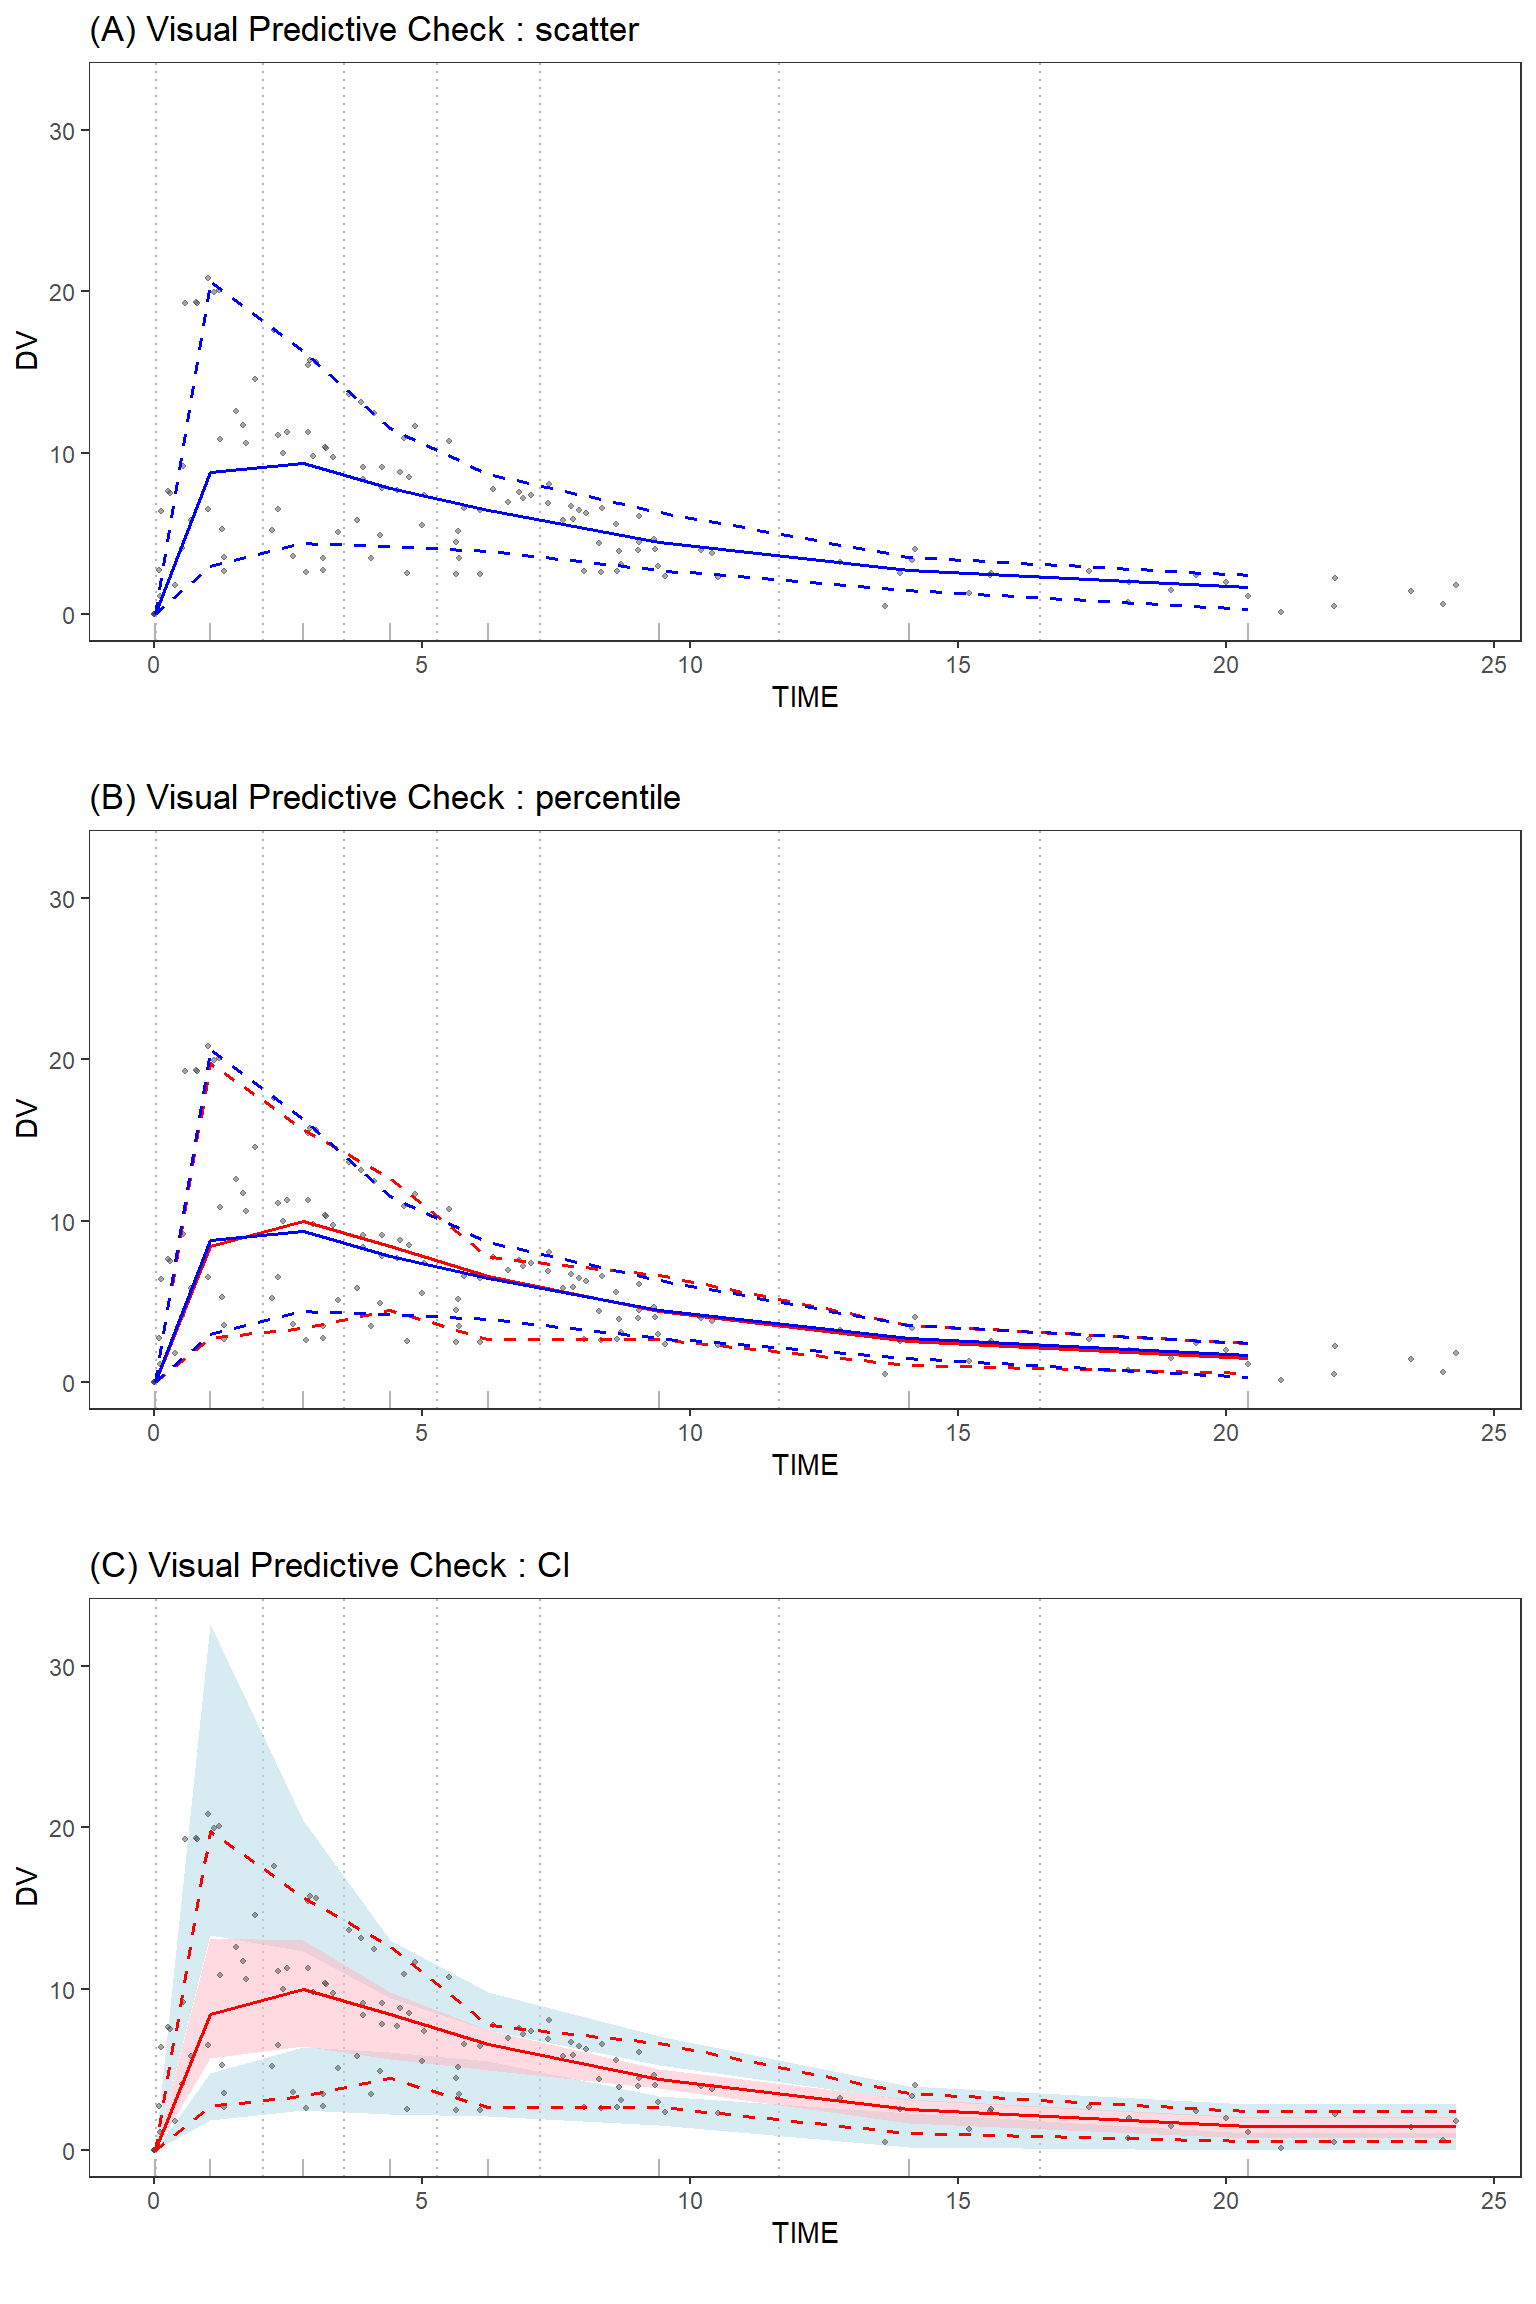
\includegraphics[width=4in,height=6in]{plotPNG/Fig0-1.png}
\label{Fig0}
\end{figure}


\hypertarget{aqrVPC}{%
\subsubsection{Additive quantile regression VPC}\label{aqrVPC}}

To overcome the difficulties of making bins as well as determining the number of bins,
\cite{jamsen2018regression} used additive quantile regression to calculate the quantiles of the observed and simulated data. This regression method makes it possible to estimate quantiles without discrete binning, which is especially useful when the data are insufficient, irregular, or inappropriate to configure the bins. To fit the additive quantile regression, we used  the \code{rqss} function in the \CRANpkg{quantreg} \citep{quantreg} package and developed the \code{aqrVPC} function to draw the VPC type plot with additive quantile regression. The right side of Figure \ref{Fig1} shows the additive quantile regression VPC plot. The solid and dashed lines represent the $10^{th}$, $50^{th}$, and $90^{th}$ additive quantile regression lines of the observed data, and the pink and light blue areas represent the confidence areas of the additive quantile regression lines of the simulated data. Lines and areas in the additive quantile regression VPC plot are much smoother than those in the original VPC plot.

\begin{figure}
\caption{The additive quantile VPC plot.  Dots indicate the observed data. The solid and dashed blue lines represent the $10^{th}$, $50^{th}$, and $90^{th}$ percentiles of the simulated data. The solid red line represents the $50^{th}$ percentile line. Light blue and pink areas represent the 95\% confidence areas of the $10^{th}$, $50^{th}$ and $90^{th}$ percentile lines.}
\centering
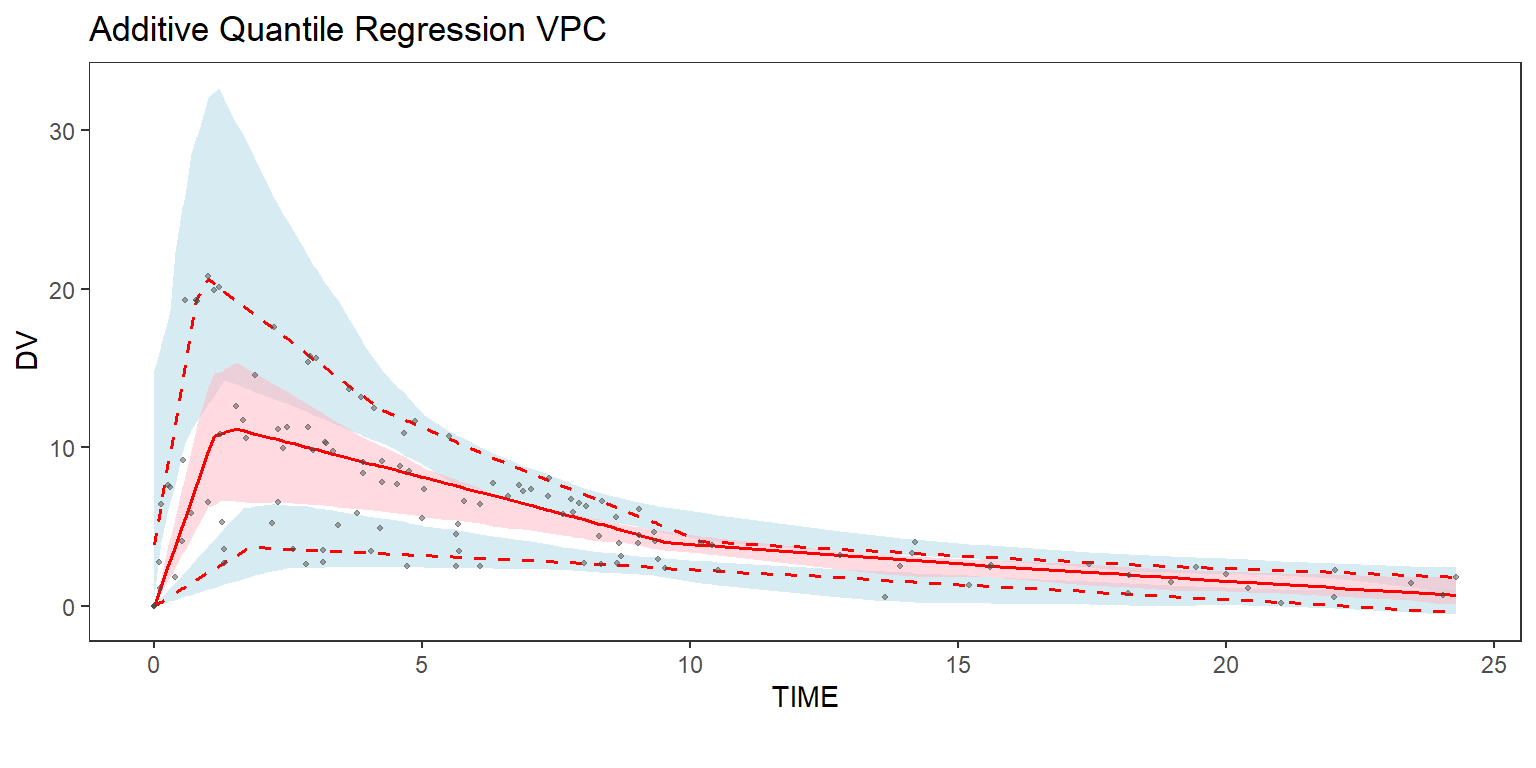
\includegraphics[width=4in,height=2in]{plotPNG/Fig1-1.png}
\label{Fig1}
\end{figure}



\hypertarget{bootVPC}{%
\subsection{Bootstrap VPC}\label{bootVPC}}

The bootstrap VPC \citep{post2008extensions} compares the distribution of the simulated data to the distribution of the bootstrap samples drawn from the observed data.
This plot reflects the uncertainty of the observed data and allows for more objective comparisons with the predicted median.

Figure \ref{Fig4} shows the bootstrap VPC plot using \code{bootVPC}.  The solid and dashed blue lines represent the $10^{th}$, $50^{th}$, and $90^{th}$ percentiles of the simulated data. The solid red line represents the $50^{th}$ percentile line, and the pink areas represent the 95\% confidence areas of the $50^{th}$ percentile line, calculated from the bootstrap samples of the observed data. If the solid blue line and the solid red line are similar, the solid blue line is in the pink area, and the pink area is located between two dashed blue lines,
then this is evidence that the fitted model fit the observed data well.


\begin{figure}
\caption{The bootstrap VPC plot. Dots indicate the observed data. The solid and dashed blue lines represent the $10^{th}$, $50^{th}$, and $90^{th}$ percentiles of the simulated data. The solid red line represents the $50^{th}$ percentile line, and the pink areas represent the 95\% confidence areas of the $50^{th}$ percentile line, calculated from the bootstrap samples of the observed data.}
\centering
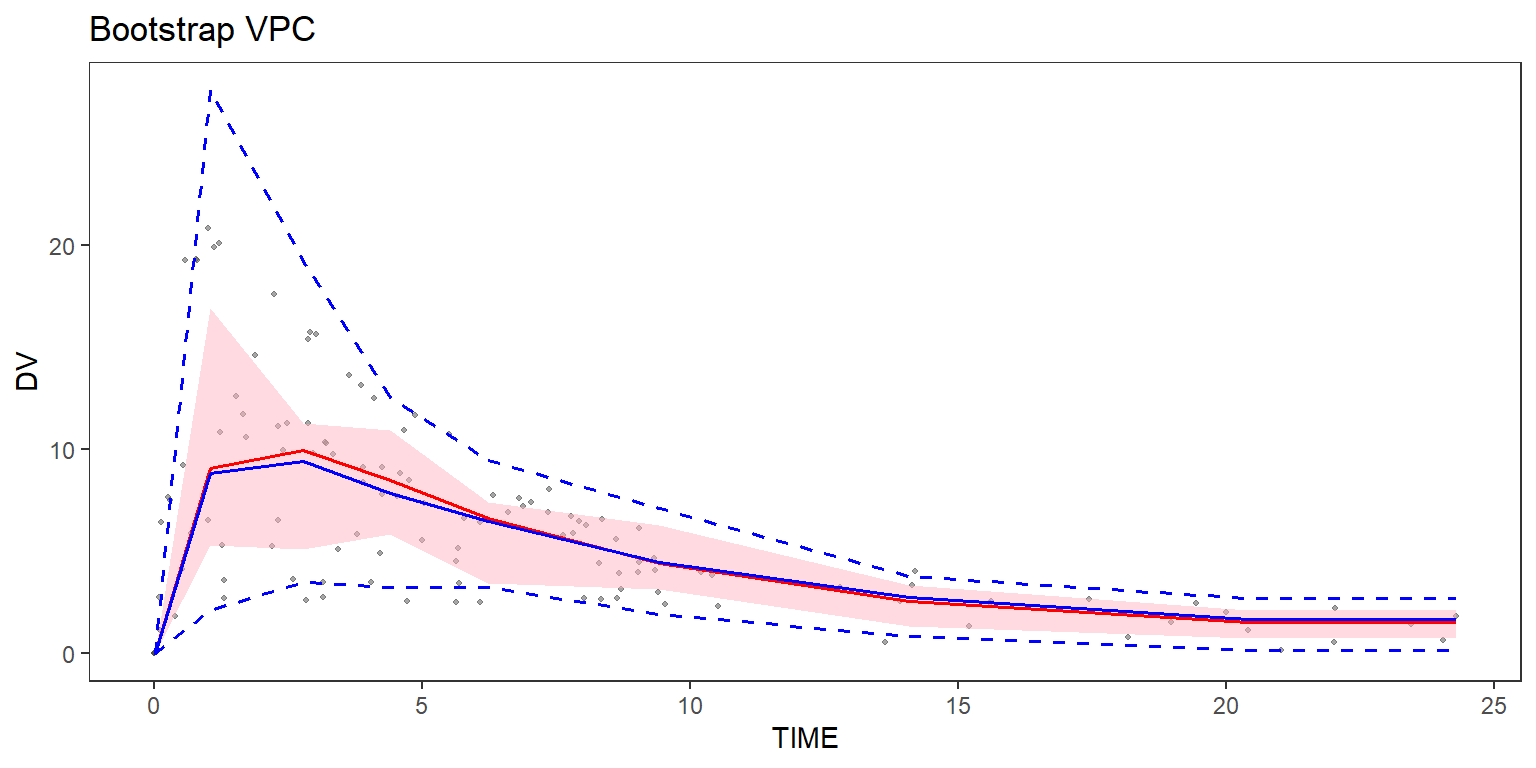
\includegraphics[width=4in,height=2in]{plotPNG/Fig2-1.png}
\label{Fig4}
\end{figure}


\hypertarget{asVPC}{%
\subsubsection{Average shifted VPC}\label{asVPC}}

Even though binning mitigates the problem with highly irregular data, the VPC plot still has a precision problem with sparse data. In this paper, we propose a new approach to draw the adapted VPC plot from the average shifted histograms \citep{scott1985ash}.
A histogram is a widely used method for displaying the density of a single continuous variable. However, histograms can look quite different based on different choice of bin width and anchor.
This requires computing an optimal bin width.
To overcome the problem with the choice of bin width and to obtain smoother estimates,  \cite{scott1985ash} proposed the averaged shifted histogram (ASH). The idea behind ASH is to make $K$ different histograms with different anchors and to combine them via a weighted average. For each histogram, the starting point is shifted by $d/K$, where $d$ is the width of the bin. We extend this idea to the VPC graph and propose the average shifted visual predictive check (asVPC) plot.

%\noindent
%\textbf{Making bins}

The binning of the VPC varies from the traditional binning in a histogram. The width of the bins is determined such that each bins contains the same, fixed number of observations, and as such the width of each bin is different. To apply the ASH idea to the VPC, we divide our data into $K*B$ bins along with the independent variable, where each bin has a different width but the same number of observations. Here, $B$ is the number of the original bins in the VPC plot, and $K$ is the number of the histograms averaged in the asVPC plot.

%\noindent
%\textbf{Combining results from each bin}

To draw the VPC plots, the following information is needed from each bin:

\begin{itemize}
\item[(A)] the median of the independent variable and percentiles of the dependent variable of the observed data.
\item[(B)] the median of the independent variable and percentiles of the dependent variable of the simulated data.
\item[(C)] 95$\%$ confidence interval of percentiles (usually $10^{th}$, $50^{th}$, and $90^{th}$ percentiles) of the dependent variable, calculated from the simulated data.
\end{itemize}

These values are also needed to produce confidence areas and percentile lines in the asVPC plot. Furthermore, additional steps are needed for asVPC. To find the median of the independent variable and percentiles of the dependent variable using the ASH algorithm, the following procedures are needed:

\begin{enumerate}
\item Divide the independent variable into $N=K*B$ bins.
\item For $i = 1, \cdots, N$,
\begin{enumerate}
\item If $i < K$, combine $bin_1, \cdots, bin_{i+K-1}$\\
else if  $K\le i\le N-K$ , combine  $bin_{i-K+1}, \cdots, bin_{i+K-1}$\\
else if  $N-K < i$ , combine $bin_{i-K+1}, \cdots, bin_N$
\item Calculate the median of the independent variable and the weighted percentiles of the dependent variable in the combined bin
 \end{enumerate}
\item Collect the medians of the independent variable and the weighted percentiles of the dependent variable from 2, and connect them to the lines.
\end{enumerate}

We can implement (A) and (B) by applying these procedures separately to the observed and simulated data. Additionally, (C) can be implemented using these procedures for each simulated dataset. First, we find the weighted percentiles, combine the results from each simulated dataset, and then calculate the 95$\%$ confidence intervals of each percentile. Using these three quantities (A), (B), and (C), we can draw the VPC type plot with the ASH approach, producing the asVPC plot.

\vspace{0.1in}
\noindent
\textbf{Determining the weights}

In the asVPC plot, the observations in each bin are combined using weights. Typically, the data near the center of the integrated bin have higher weights, and the data far from the center have smaller weights. This idea is used in the ASH algorithm as well as the density estimation literature. We suggest two different ways to apply weights for the asVPC calculation.


\begin{itemize}
\item	Bin-related weight: For each bin in the combined bin, K-1 bins in both directions have weights and the other bins have no weight. Use $\frac{1}{K}$, $\cdots$, $\frac{i-1}{K}$, $\cdots$, $\frac{K-1}{K}$, $1$, $\frac{K-1}{K}$, $\cdots$, $\frac{i-1}{K}$, $\cdots$, $\frac{1}{K}$ as weights for 2K-1 bins. This approach is the same as the original ASH approach.
\item	Distance-related weight: Use the reciprocal of the distance from the center of the independent variable in each combined bin so that the points near the center have higher weights and the points far from the center have lower weights.
\end{itemize}

Figure \ref{Fig3} shows the results from the \code{asVPC} function using bin-related weights and distance-related weights. The solid and dashed lines represent the average shifted quantile lines of the observed data, and the pink and light blue areas represent the confidence areas of the simulated data. The lines in the asVPC plot are smoother than those in the original VPC plot, and the confidence areas in the asVPC plot are thinner than those in the original VPC plot.


\begin{figure}
\caption{The average shifted VPC plot. Dots indicate the observed data. The solid line represents the 50th quantiles of the observed data, and dashed lines represent the $10^{th}$ and $90^{th}$ percentiles of the observed data. Light blue and pink areas represent the 95\% confidence areas of the $10^{th}$, $50^{th}$, and $90^{th}$ percentiles.}
\centering
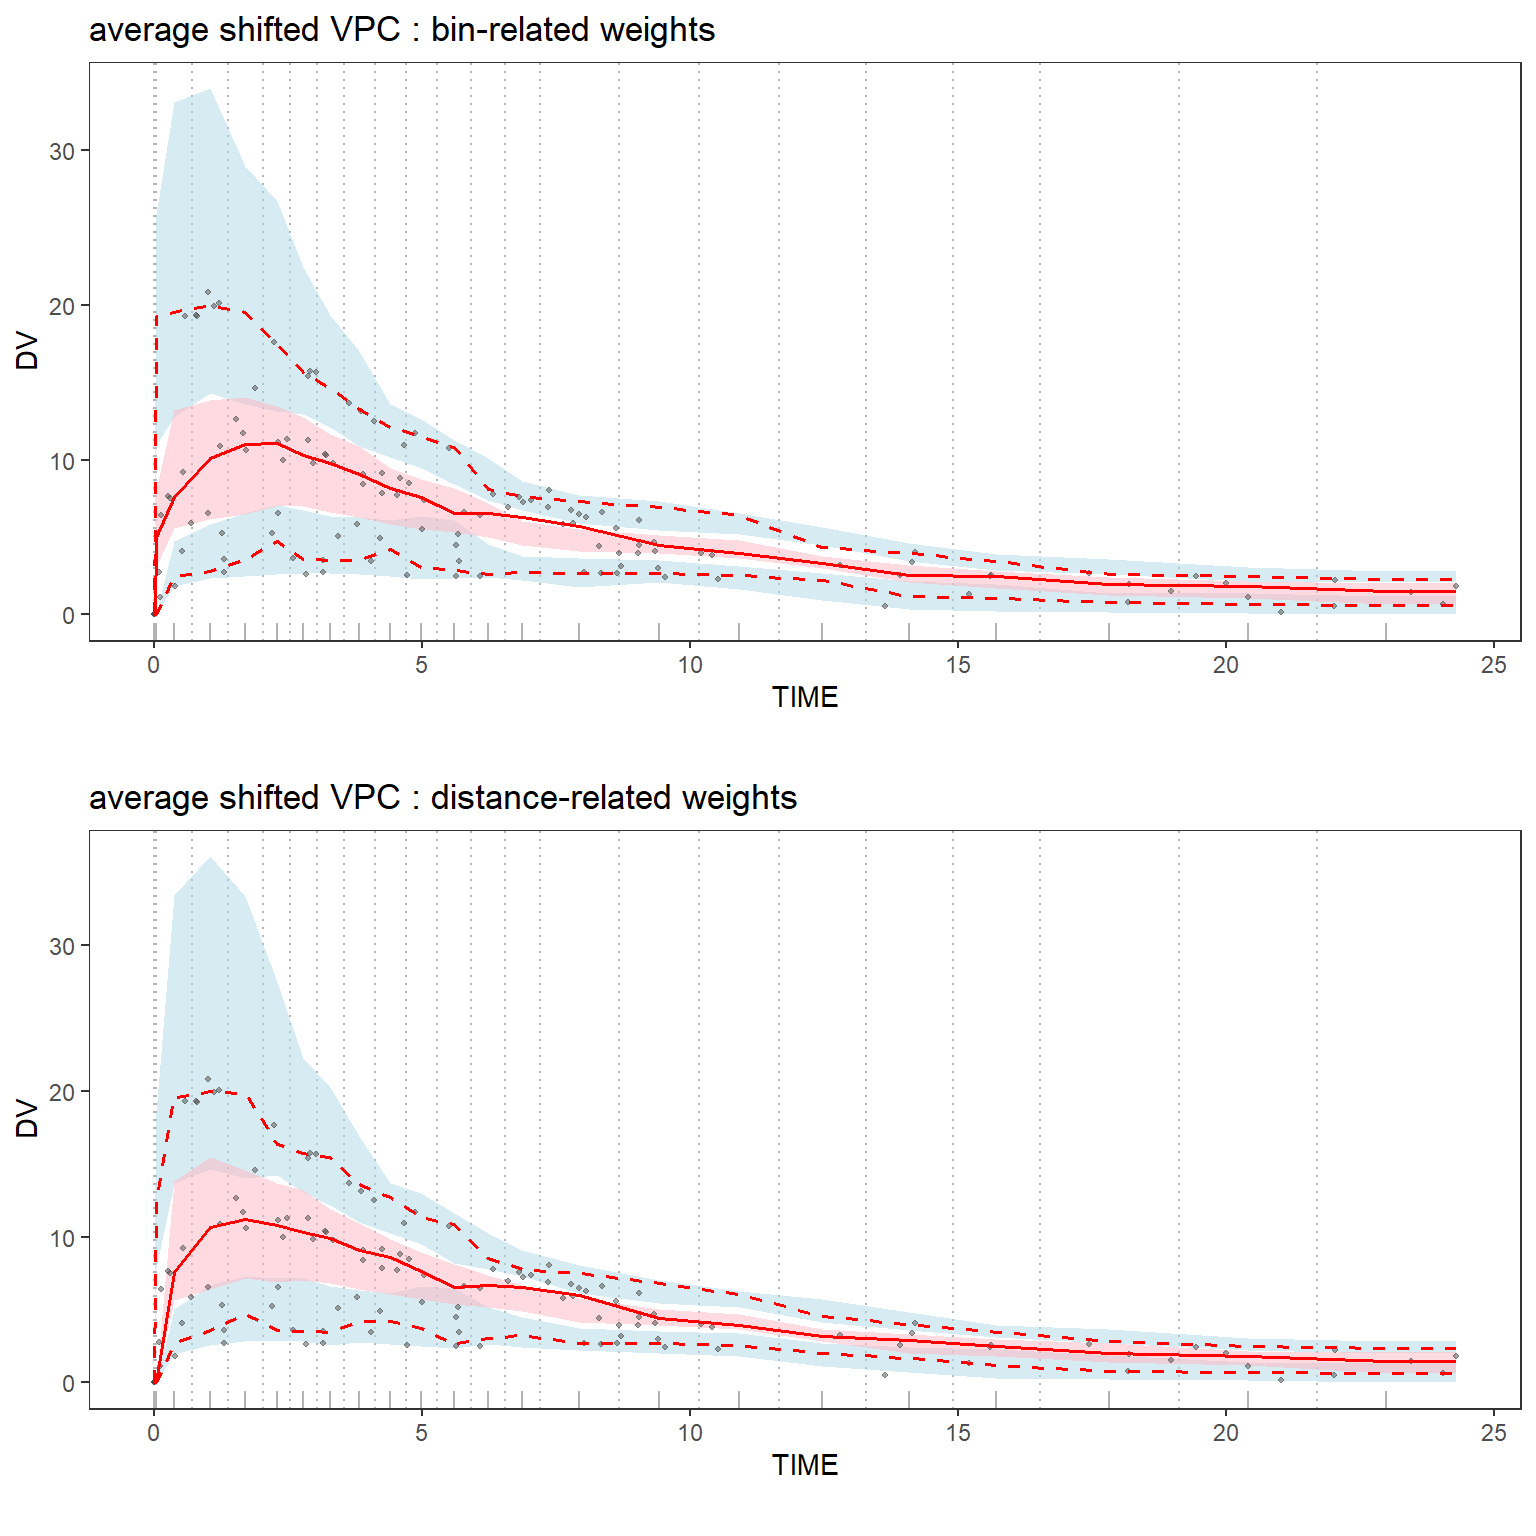
\includegraphics[width=4in,height=4in]{plotPNG/Fig3-1.png}
\label{Fig3}
\end{figure}

\hypertarget{MS}{%
\section{Validation in the model space}\label{MS}}

To validate the fitted model in the model space, we need to choose appropriate statistics to visualize and describe them in the model space. In \pkg{nlmeVPC}, we use the same statistics, that is quantiles, as the VPC plot in the data space, and compare them in two ways - numerically and visually. The numerical predictive check and the coverage plot are two commonly used methods in pharmacometrics. However, there is a limitation to detecting the illness of the fitted model. These methods combine the results of all ranges of the independent variable, and it is helpful to see the overall fitness. However, it is not easy to detect the detailed discrepancy between the fitted model and the observed data. To overcome this limitation, we developed a new plot, the coverage detailed plot, to compensate for the shortness of the coverage plot.

\hypertarget{NPC}{%
\subsection{Numerical predictive check}\label{NPC}}

The VPC plot visually compares the observed data to the simulated percentiles in the data space. On the other hand, the numerical predictive check (NPC; \citealp*{wang2012standardized}; \citealp*{karlsson2007diagnosing})
numerically compares the observed data to the simulated data. For a given level of prediction (for example, 90\%), the predicted interval is calculated using the simulated data, and the number of the observed data points outside of the prediction interval is counted, both below the lower bound and above the upper bound. The expected number of points below the lower bound of the predicted interval (for example, 5\% of observations) is also calculated and compared to the observed number. If these two numbers are similar, the suggested model is suitable \citep{maharaj2019pitfalls}.

\code{NumericalCheck} provides information summarizing the results of the NPC for various prediction levels.
 {\tt PI} is the prediction level $\times$ 100 and {\tt n} is the number of observations.
 {\tt ``Expected points below PI''} and {\tt ``Expected points above PI''} are respectively the expected numbers below and above the PI; {\tt ``points below PI''} and {\tt ``points above PI''} respectively represent the numbers of points below and above the PI;
 {\tt ``95\%CIBelowFrom(\%)''} and {\tt ``95\%CIBelowTo(\%)''} represent the 95\% confidence interval of {\tt ``points below PI(\%)''}; and {\tt ``95\%CIAboveFrom(\%)''} and {\tt ``95\%CIAboveTo(\%)''} represent the 95\% confidence interval of {\tt ``points above PI(\%)''}. If {\tt ``points below PI(\%)''} is in the
95\% confidence intervals of {\tt ``points below PI(\%)''} and is similar to {\tt ``Expected points below PI''}, and if
  {\tt ``points above PI(\%)''} is in the
95\% confidence intervals of {\tt ``points above PI(\%)''} and is similar to {\tt ``Expected points above PI''}, this is the evidence that the fitted model explains the data well.

\begin{Schunk}
\begin{Sinput}
> NumericalCheck(origdata,simdata,pred.level=c(0,0.2,0.4,0.6,0.8,0.9),N_xbin=8)$NPC
\end{Sinput}
\begin{Soutput}
  PI   n Expected points below PI points below PI points below PI(%)
1  0 132                     66.0              57           43.18182
2 20 132                     52.8              46           34.84848
3 40 132                     39.6              37           28.03030
4 60 132                     26.4              27           20.45455
5 80 132                     13.2              17           12.87879
6 90 132                      6.6               7            5.30303
  95%CIBelowFrom(%) 95%CIBelowTo(%) Expected points above PI points above PI
1        35.6060606        56.81818                     66.0              63
2        26.8750000        48.88258                     52.8              49
3        20.4545455        36.76136                     39.6              35
4        11.3636364        26.15530                     26.4              28
5         3.7878788        16.66667                     13.2              12
6         0.3598485        10.64394                      6.6               5
  points above PI(%) 95%CIAboveFrom(%) 95%CIAboveTo(%)
1          47.727273         34.090909       55.303030
2          37.121212         25.359848       46.609848
3          26.515152         16.666667       36.003788
4          21.212121         10.965909       25.000000
5           9.090909          2.632576       15.549242
6           3.787879          1.117424        8.333333
\end{Soutput}
\end{Schunk}

\hypertarget{coverage}{%
\subsubsection{Coverage plot}\label{coverage}}

 The result of the NPC is a table with many values, which, while useful, can be difficult to parse visually. The coverage plot \citep{karlsson2008tutorial} was developed to help visually check the fitted model with the NPC result.
In each level of the predicted interval, the ratios between the expected number of data points (Exp) outside the prediction interval and the observed number of data  points (Obs)
outside the prediction interval are calculated. These ratios are calculated separately for the upper and lower bound of the prediction interval. For example, when the prediction level is 90, a 90\% prediction interval is used, and 10\% of the observations are expected to locate outside this prediction interval. To be more precise, 5\% of observations are expected to be above the upper limit, and 5\% of observations are expected to be below the lower limit.

The coverage plot with the NPC result can diagnose a model using multiple prediction intervals. The X-axis represents the prediction level, and the Y-axis represents Obs/Exp. The closer Obs/Exp is to 1, the more appropriate the model is. Furthermore, the confidence intervals of Obs/Exp values are obtained using simulated data and then expressed together in the plot for a more objective comparison. This plot can provide more information than the VPC plot, which interprets only a couple of quantiles - usually the 10\%, 50\%, and 90\% percentiles.

The \pkg{xpose4} package \citep{keizer2013modeling} provides a coverage plot. However,
to draw the coverage plot using \pkg{xpose4}, PsN \citep{lindbom2004perl} software is needed to calculate  the NPC result. Therefore, we developed \code{coverageplot} to draw the coverage plot using the results from \code{NumericalCheck}.

Figure \ref{Fig5}(A) shows the coverage plot. The X-axis shows the level of the prediction interval. The Y-axis show the ratio between the observed number of data and the expected number of data of the lower and upper parts in each level of the prediction interval. The white line is the reference line, and the gray area represents the confidence areas of the ratios in each prediction level. If the solid lines are near the white line or in the gray area, we can conclude that the suggested model is suitable.


\begin{figure}
\caption{The coverage plot and the coverage detailed plot for the 80\% prediction interval. In the coverage plot, the X-axis is the level of the prediction interval. The Y-axis is the ratio between the number of observed data and the number of expected data of the lower and upper parts in each level of the prediction interval. The white line is the reference line, and the gray area represents the confidence area of the ratios. If the solid lines are near the white line, we can conclude that the suggested model is suitable. In the coverage detailed plot, the white dots represent the expected percentages of lower and upper prediction intervals of, 10\%, and 90\%, respectively. The upper and lower percentages of observation in each time bin are darker gray. }
\centering
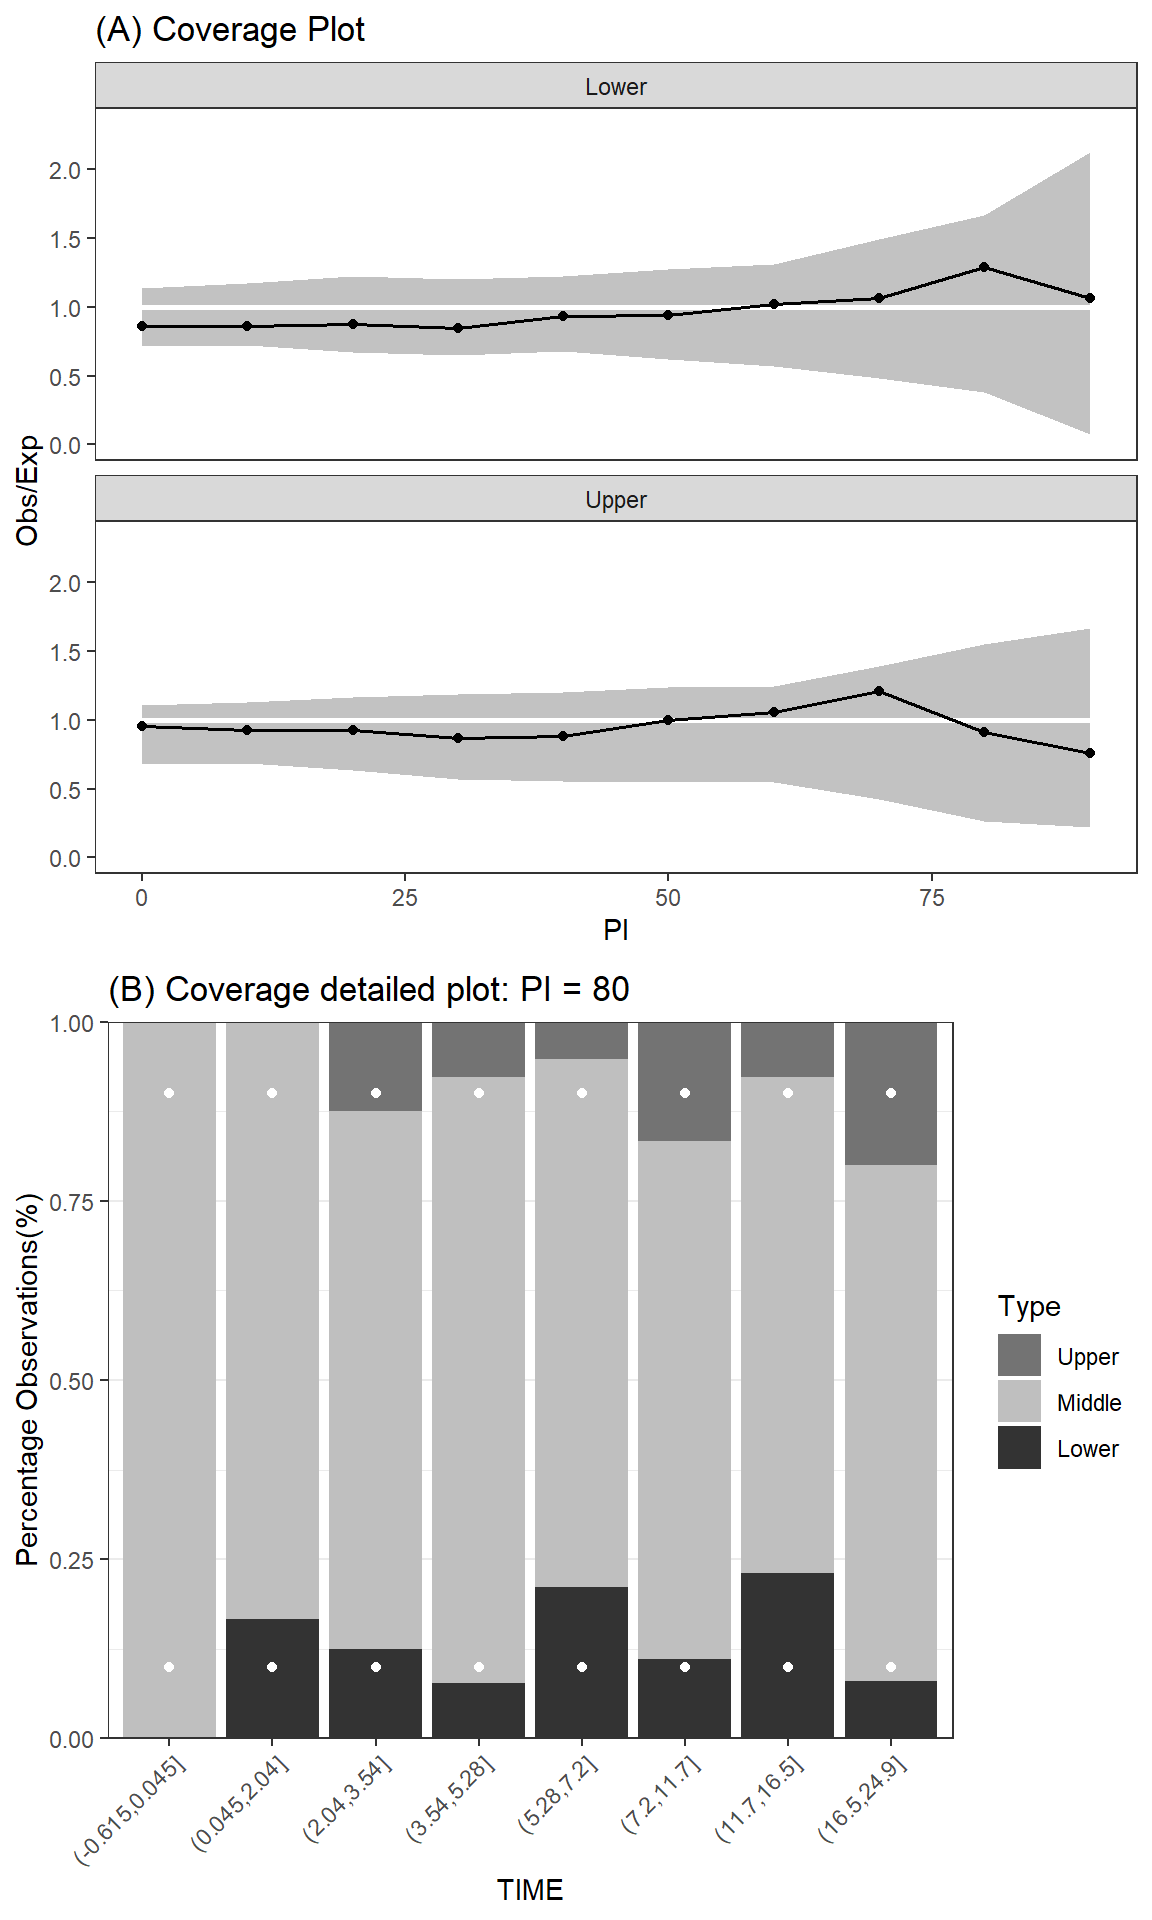
\includegraphics[width=3in,height=5in]{plotPNG/Fig4-1.png}
\label{Fig5}
\end{figure}


\hypertarget{coverageDetail}{%
\subsection{Coverage detailed plot}\label{coverageDetail}}

Unlike the VPC plot, which represents the data space, the information in the observed data space does not come together in the coverage plot, which makes it difficult to determine whether the model is overestimated, underestimated, or adequate in the specific region of the data space. To overcome this limitation of the coverage plot, we propose a new method called the coverage detailed plot.
 The percentages of observations above the prediction interval are calculated in each bin of the independent variable. Additionally, the percentages of observations below the prediction interval are calculated. The white dots in the plot represent the expected percentages. If the percentages of upper and lower observations are near the white dots,  we can conclude that the suggested model is suitable for the specific prediction interval.

Figure \ref{Fig5}(B) is the result of \code{coverageDetailplot} when the prediction level is 80\%. The white dots represent the expected percentages of the lower and upper the prediction intervals, 10\%, and 90\%, respectively. The upper and lower percentages of observation in each time bin are shown in darker gray. The left bin(before 0.045 hours) shows all light gray in the coverage detailed plot, and it is quite different patterns from the expected one. However, it is mainly due to the characteristics of this example data. All observations in this bin are 0. It makes the lower and upper bound of the prediction interval all 0, and the lower and upper percentages become 0.




\hypertarget{QVPC}{%
\subsection{Quantified VPC}\label{QVPC}}

\cite{post2008extensions} proposed the quantified VPC (QVPC). It expanded the existing VPC, including information about missing data.
The QVPC plot visually represents actual and unavailable observations around the predicted medians through the form of percent, regardless of the observed data's density or shape. Here, ``unavailable observations'' refer to all kinds of missing values and unobserved data that occur for various reasons, including deviations and unexpected omissions.

If the model is appropriate, observations at each time bin are allocated randomly around the predicted median of the model. In the QVPC plot, white dots represent the model's predicted median in each bin. If the borderlines above and below are close to the white dots, we can conclude that the fitted model describes the observed data well.

Figure \ref{Fig7} shows the result of \code{quantVPC}.  The darker gray areas represent the percentages below the median. The lighter gray areas represent the percentage above. The brightest gray areas represent the percent unavailable in each time bin. The white dots represent the ideal location where the above and the below percentages meet. In this example, there is no missing value.

\begin{figure}
\caption{The quantified VPC plot. The darker gray areas represent the percentages below the median, the lighter gray areas represent the percentage above, and the brightest gray areas represent the percent unavailable in each time bin. The white dots represent the ideal location where the above and the below percentages meet.}
\centering
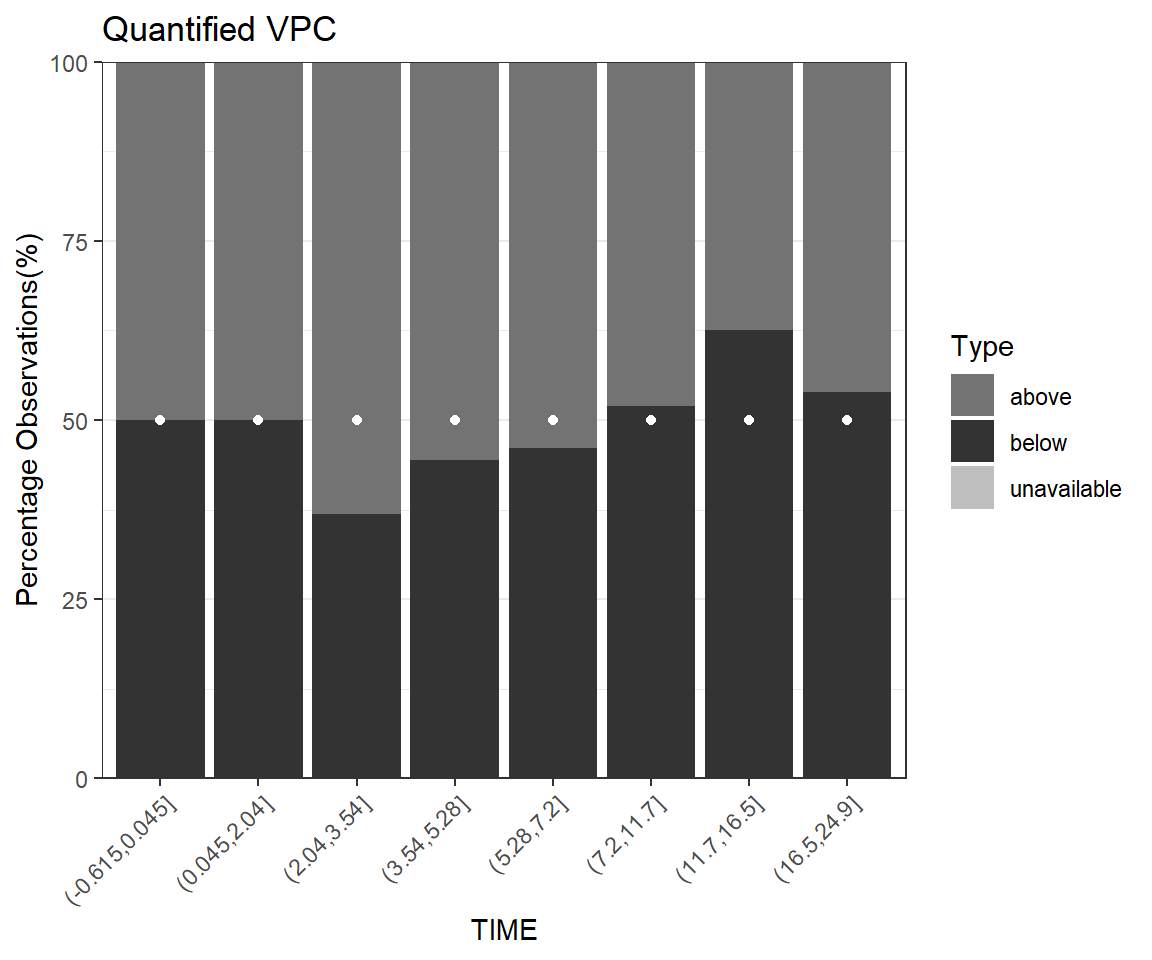
\includegraphics[width=3in,height=2.5in]{plotPNG/Fig5-1.png}
\label{Fig7}
\end{figure}

%\newpage
%\section{The nlmeVPC package: structure and functionality}
%Table \ref{table1} shows the list of functions and table \ref{table2} shows the list of arguments used in the functions of \code{nlmeVPC}.

% Insert table

\begin{table}
\centering
\begin{tabular}{ll}
  \hline
  % after \\: \hline or \cline{col1-col2} \cline{col3-col4} ...
  Function & Description \\\hline
  \code{VPCgraph} & draw the original VPC plot \\
  \code{aqrVPC} & draw the additive quantile regression VPC plot \\
  \code{bootVPC} & draw the bootstrap VPC plot \\
  \code{asVPC} & draw VPC using ASH method \\ \hline
  \code{NumericalCheck} & calculate the numbers to check coverage in each prediction level \\
  \code{coverageplot} & plot the result of NumericalCheck \\
  \code{coverageDetailplot} & plot for checking specific prediction level \\
  \code{quantVPC} & plot for the quantified VPC \\\hline
\end{tabular}
\caption{List of functions to check the validity of model with the observed data and the simulated data}
\label{table1}
\end{table}


\begin{table}
\centering
\begin{tabular}{ll}
  \hline
  % after \\: \hline or \cline{col1-col2} \cline{col3-col4} ...
  Argument           & Description  \\\hline
 \code{orig\_data}    & A data frame of original data with X and Y variable\\
 \code{sim\_data}     & A matrix of simulated data with only Y values collected\\
 \code{type}          & Type of VPC graph; "CI", "percentile", or "scatter"\\
 \code{weight\_method} & The way to put weights in \code{asVPC}; "bin" or "distance"\\
 \code{N\_xbin}       & Number of bins in X variable \\
 \code{probs}         & A numeric vector of probabilities\\
 \code{conf.level}    & Confidence level of the interval\\
 \code{X\_name}       & Name of X variable in \code{orig\_data}\\
 \code{Y\_name}       & Name of Y variable in \code{orig\_data}\\
 \code{subject\_name} & Name of subject variable in \code{orig\_data}\\
 \code{MissingDV}     & Name of missing indicator variable in \code{orig\_data}\\
 \code{DV\_point}     & Draw point (X, Y) in the plot if TRUE; omit if FALSE\\
 \code{CIvpc\_type}   & Type of CI area in VPC graph; "line" or "segment"\\
 \code{bin\_grid}     & Draw grid lines for binning in X variable if TRUE; omit if FALSE\\
 \code{plot\_caption} & Put caption with additional information if TRUE; omit if FALSE\\
 \code{plot\_flag}    & Draw plot if TRUE; generate data for drawing plot if FALSE\\
 \code{linesize}      & Size of line in the plot\\
 \code{pointsize}     & Size of point in the plot\\
 \code{captionsize}   & Size of caption \\
 \code{maxK}          & The maximum number of bins\\
 \code{Kmethod}       & The way to calculate the penalty in automatic binning; "cluster" or "kernel"\\
 \code{beta}          & Additional parameter for automatic binning, used in \code{optK} function\\
 \code{lambda}        & Additional parameter for automatic binning, used in \code{optK} function\\\hline
\end{tabular}
\caption{Summary of the arguments of functions in \pkg{nlmeVPC}.}
\label{table2}
\end{table}


\hypertarget{nlmeVPCPKG}{%
\section{The nlmeVPC package: structure and functionality}\label{nlmeVPCPKG}}


Table \ref{table1} shows the list of functions and Table \ref{table2} shows the list of arguments used in the functions of \pkg{nlmeVPC}. The following codes are for Figure \ref{Fig0} to Figure \ref{Fig7}.

\begin{Schunk}
\begin{Sinput}
> library(nlmeVPC)
> data(origdata)
> data(simdata)
> optK(origdata$TIME)$K
\end{Sinput}
\begin{Soutput}
[1] 8
\end{Soutput}
\begin{Sinput}
> # Figure 1
> VPCgraph(origdata,simdata,N_xbin=8,type="scatter")
>     + labs(title="(A) Visual Predictive Check : scatter",caption="")
> VPCgraph(origdata,simdata,N_xbin=8,type="percentile")
>     + labs(title="(B) Visual Predictive Check : percentile",caption="")
> VPCgraph(origdata,simdata,N_xbin=8,type="CI")
>     + labs(title="(C) Visual Predictive Check : CI",caption="")
> # Figure 2
> aqrVPC(origdata,simdata)+labs(caption="")
> # Figure 3
> bootVPC(origdata,simdata,N_xbin=8)
> # Figure 4
> asVPC(origdata,simdata,type="CI",N_xbin=8,N_hist=3,weight_method="bin")+
>    labs(caption="")
> asVPC(origdata,simdata,type="CI",N_xbin=8,N_hist=3,weight_method="distance")+
>    labs(caption="")
> # Numerical Predictive Check
> NumericalCheck(origdata,simdata,N_xbin=8,pred.level=c(0,0.2,0.4,0.6,0.8,0.9))$NPC
> # Figure 5
> coverageplot(origdata,simdata,N_xbin=8)+ggtitle("(A) Coverage Plot")
> coverageDetailplot(origdata,simdata,N_xbin=8,predL=0.8) +
>    ggtitle("(B) Coverage detailed plot: PI = 80")
> # Figure 6
> quantVPC(origdata,simdata)
\end{Sinput}
\end{Schunk}


We use an example to show how to use functions in \pkg{nlmeVPC} and how they work.


\hypertarget{Example}{%
\subsection{Example}\label{Example}}

The \code{origdata} in \pkg{nlmeVPC} is from an experiment on the pharmacokinetics of theophylline. Twelve patients were given oral doses of theophylline, and blood concentrations were measured at 11 time points over the next 25 hours. Each patient had different time points.
We consider the following first-order absorption one-compartment model:

\begin{equation}
y_{ij}= \frac{Amt_i * Ke_i *Ka_i}{Cl_i} \left(\exp( -Ke_i * TIME_{ij})-\exp(-Ka_i * TIME_{ij})\right) +\varepsilon_{ij}.
\end{equation}

In this model, $y_{ij}$ is the theophylline concentration at $TIME_{ij}$ after an initial dose of $Amt_i$. The pharmacokinetic parameters are the absorption rate constant $Ka$, the elimination rate constant $Ke$, and the clearance $Cl$.
In this example, two different models are fitted and diagnosed using functions in the \pkg{nlmeVPC} package. In Model 1, $Ka$ and $Cl$ are considered as random effects. In Model 2, $Ke$ is considered as random effect, and $Ka$ and $Cl$ are considered only as a fixed effect. The \CRANpkg{nlme} \citep{nlme} and \CRANpkg{nlraa} \citep{nlraa}  packages are used to fit the nonlinear mixed models and to generate the simulated data from the fitted model.

\begin{Schunk}
\begin{Sinput}
> library(nlme)
> library(nlraa)
> library(nlmeVPC)
> data(origdata)
> origdataT <- groupedData(DV~TIME|ID,origdata)
> # Model 1
> T.nlme <- nlme(DV ~ exp(lKe+lKa-lCl)*AMT*
+                  (exp(-exp(lKe)*TIME) - exp(-exp(lKa)*TIME))/
+                  (exp(lKa)-exp(lKe)), data=origdataT,
+                fixed=lKa+lKe+lCl~1,
+                random=lKa+lCl~1,
+                start=c(lKe=-2,lKa=1.5,lCl=-3))
> set.seed(123456)
> sim.T <- simulate_nlme(T.nlme,nsim=100,psim=3,level=1,value="data.frame")
> simdata.T <- matrix(sim.T$sim.y,ncol=100)
> # Model 2
> F.nlme <- nlme(DV ~ exp(lKe+lKa-lCl)*AMT*
+                 (exp(-exp(lKe)*TIME) - exp(-exp(lKa)*TIME))/
+                 (exp(lKa)-exp(lKe)), data=origdataT,
+               fixed=lKa+lKe+lCl~1,
+               random=lKe~1,
+               start=c(lKe=-2,lKa=1.5,lCl=-3))
> sim.F <- simulate_nlme(F.nlme,nsim=100,psim=3,level=1,value="data.frame")
> simdata.F <- matrix(sim.F$sim.y,ncol=100)
\end{Sinput}
\end{Schunk}

\begin{Schunk}
\begin{Sinput}
> # Figure 7
> VPCgraph(origdata,simdata.T,type="CI",N_xbin=8) + labs(title="Model 1",caption="")
> VPCgraph(origdata,simdata.F,type="CI",N_xbin=8) + labs(title="Model 2",caption="")
> # Figure 8
> aqrVPC(origdata,simdata.T) + labs(title="Model 1",caption="")
> aqrVPC(origdata,simdata.F) + labs(title="Model 2",caption="")
> # Figure 9
> asVPC(origdata,simdata.T,type="CI",weight_method="distance",N_xbin=8) +
>     labs(title="Model 1",caption="")
> asVPC(origdata,simdata.F,type="CI",weight_method="distance",N_xbin=8) +
>     labs(title="Model 2",caption="")
> # Figure 10
> bootVPC(origdata,simdata.T,N_xbin=8) + labs(title="Model 1")
> bootVPC(origdata,simdata.F,N_xbin=8) + labs(title="Model 2")
> # Figure 11
> coverageplot(origdata,simdata.T,conf.level=0.9,N_xbin=8) + labs(title="Model 1")
> coverageplot(origdata,simdata.F,conf.level=0.9,N_xbin=8) + labs(title="Model 2")
> # Figure 12
> coverageDetailplot(origdata,simdata.T,predL=0.5,N_xbin=8) + labs(title="Model 1")
> coverageDetailplot(origdata,simdata.F,predL=0.5,N_xbin=8) + labs(title="Model 2")
> # Figure 13
> coverageDetailplot(origdata,simdata.T,predL=0.8,N_xbin=8) + labs(title="Model 1")
> coverageDetailplot(origdata,simdata.F,predL=0.8,N_xbin=8) + labs(title="Model 2")
> # Figure 14
> quantVPC(origdata,simdata.T,N_xbin=8) + labs(title="Model 1")
> quantVPC(origdata,simdata.F,N_xbin=8) + labs(title="Model 2")
\end{Sinput}
\end{Schunk}

Figure \ref{M11} shows the \code{VPCgraph} for Model 1 and Model 2.
The solid line represents the 50$^{th}$ percentile of the observed data, and the dashed lines represent the 10$^{th}$ and 90$^{th}$ percentiles of the observed data. In Model 1, all quantile lines (the solid and dashed lines) are in the confidence area. However, the 10$^{th}$ and 90$^{th}$ percentiles in Model 2 are mostly outside the confidence area, especially at 0 to 5 hours.

\begin{figure}
\caption{The VPC plots of Model 1 and Model 2.}
\centering
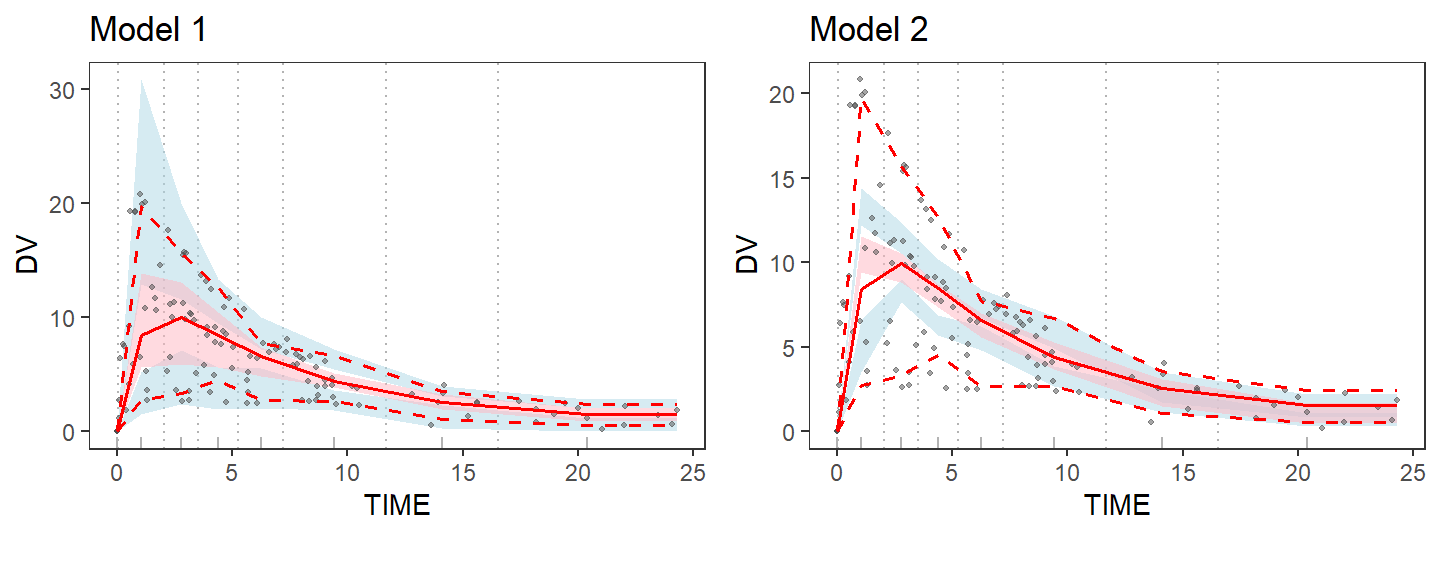
\includegraphics[width=5in,height=2in]{plotPNG/M11-1.png}
\label{M11}
\end{figure}


Figure \ref{M12} shows the results of \code{aqrVPC}, and Figure \ref{M13} shows the results of \code{asVPC} for Model 1 and Model 2. The additive quantile regression VPCs and the average shifted VPCs show similar patterns to the original VPCs. Model 1 shows all quantile lines in the confidence area, and the 10$^{th}$ and 90$^{th}$ percentiles in Model 2 are mostly outside the confidence area.

\begin{figure}
\caption{The additive quantile regression VPC plots for Model 1 and Model 2.}
\centering
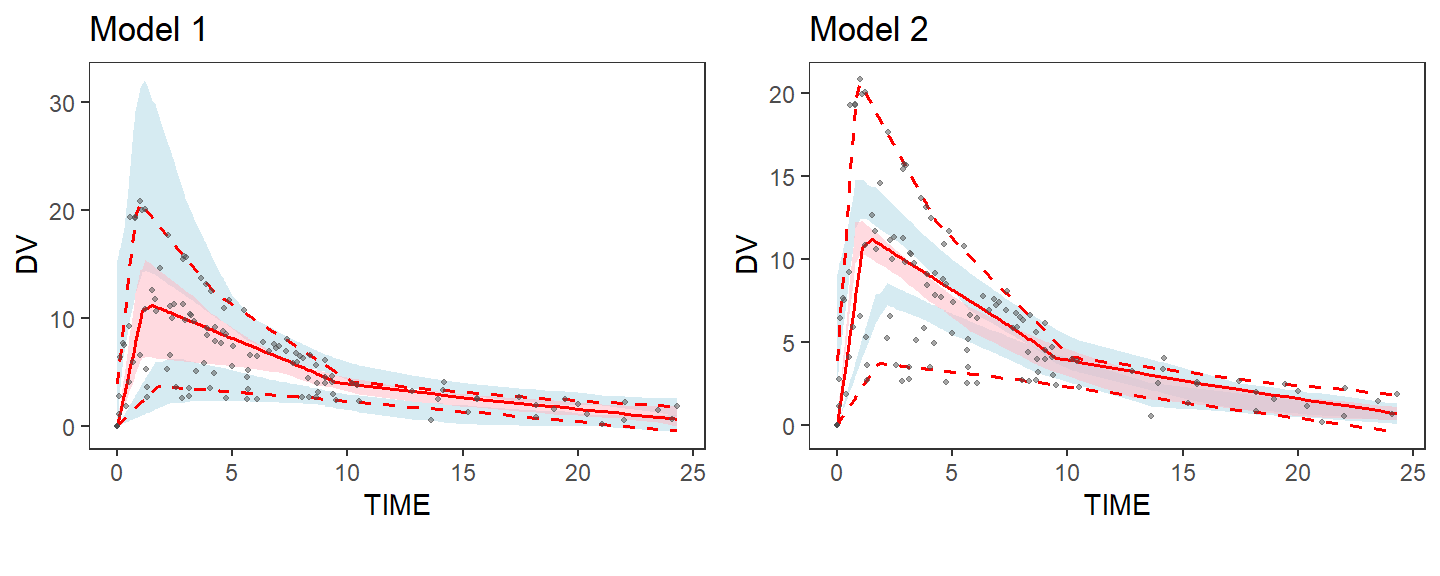
\includegraphics[width=5in,height=2in]{plotPNG/M12-1.png}
\label{M12}
\end{figure}

\begin{figure}
\caption{The average shifted VPC plots for Model 1 and Model 2.}
\centering
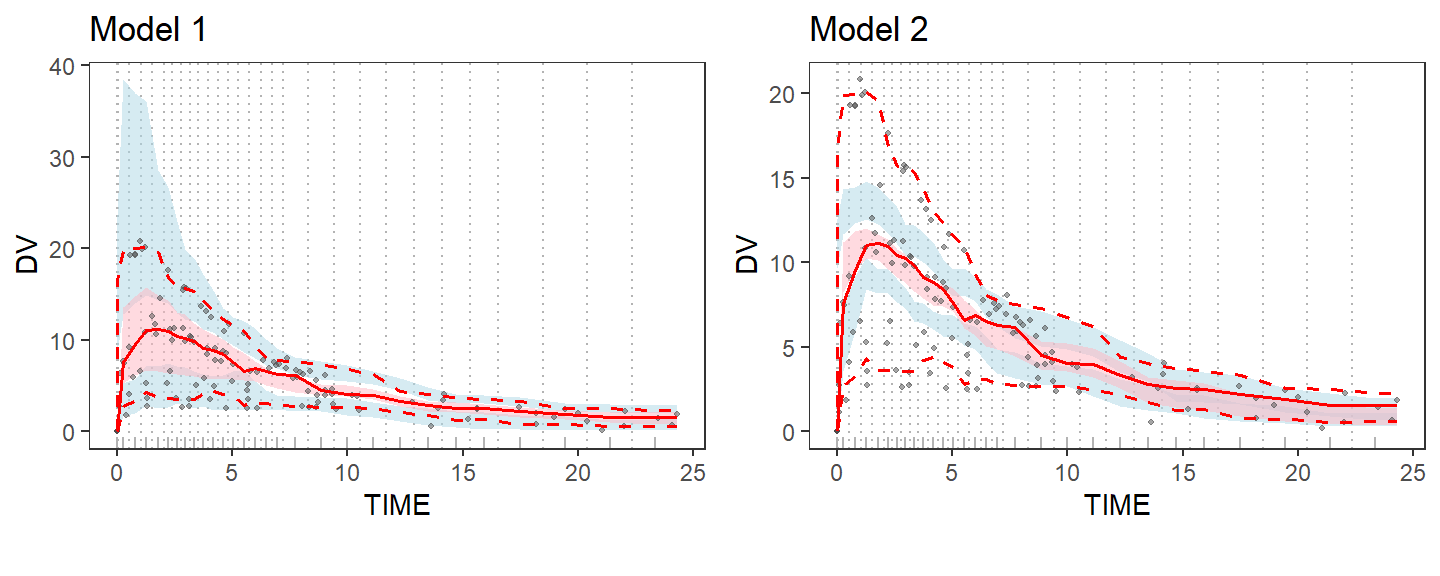
\includegraphics[width=5in,height=2in]{plotPNG/M13-1.png}
\label{M13}
\end{figure}


Figure \ref{M14} shows the results of \code{bootVPC} for Model 1 and Model 2. The solid and dashed blue lines show the $10^{th}$, $50^{th}$, and $90^{th}$ percentiles of the simulated data. The solid red line represents the $50^{th}$ percentile line of the observed data, and the pink areas represent the 95\% confidence areas of the $50^{th}$ percentile line, calculated from the bootstrap samples of the observed data.
The solid blue line is in the pink area, and the two solid red and blue lines are almost identical in both models.
The dashed blue lines in Model 1 cover most of the observed data. However, the dashed blue lines in Model 2 do not cover the observed data. Many observed data points lie outside these dashed blue lines in Model 2, especially in 0 to 10 hours.

\begin{figure}
\caption{The bootstrap VPC plots for Model 1 and Model 2.}
\centering
 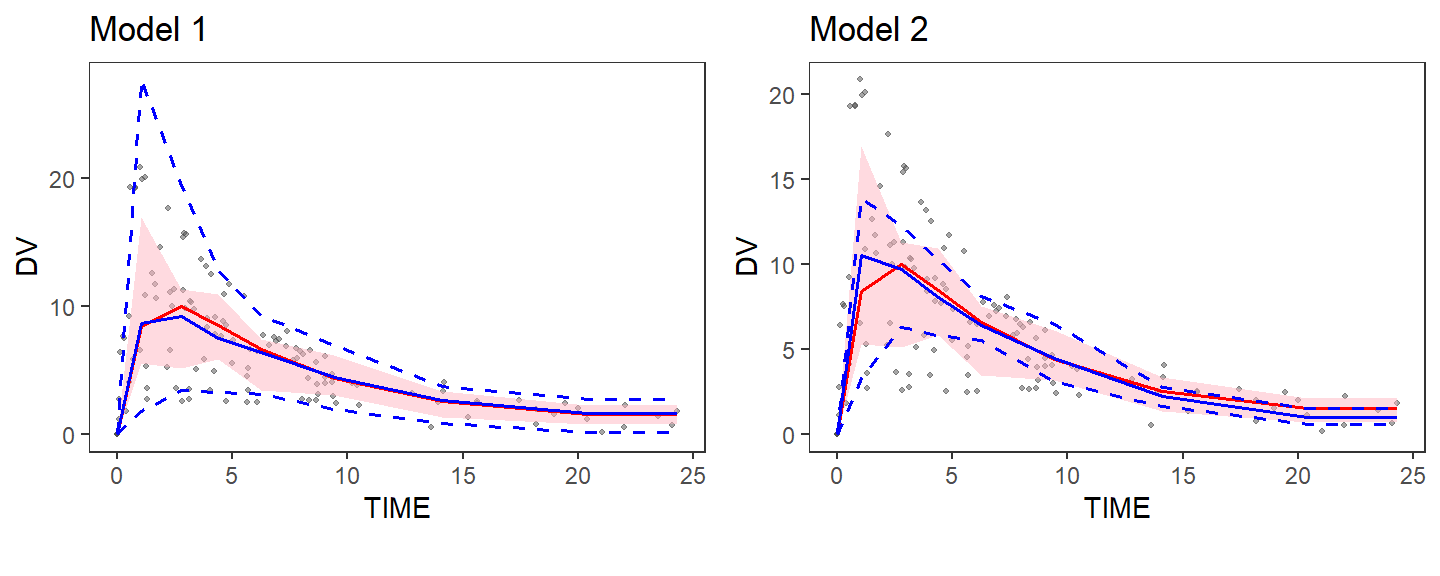
\includegraphics[width=5in,height=2in]{plotPNG/M14-1.png}
\label{M14}
\end{figure}


\begin{figure}
\caption{The coverage plots for Model 1 and Model 2.}
\centering
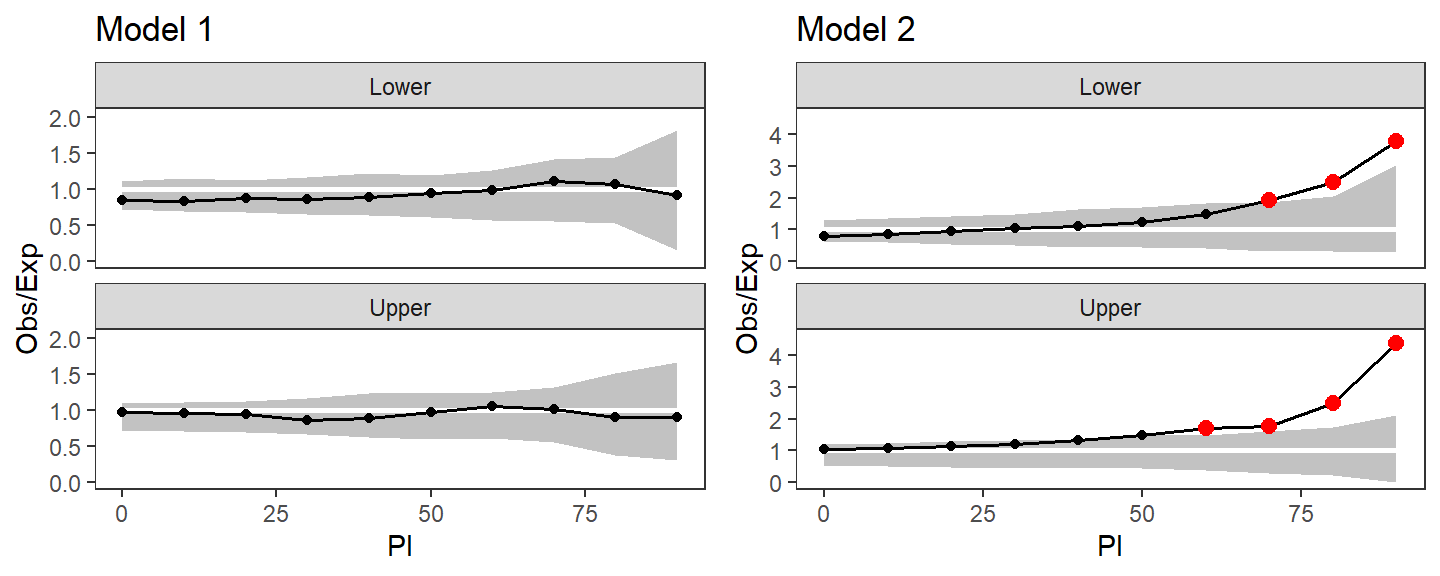
\includegraphics[width=5in,height=2in]{plotPNG/M15-1.png}
\label{M15}
\end{figure}


Figure \ref{M15} shows the  \code{coverageplot} results for Model 1 and Model 2. The lines are in the gray area and close to the white line in Model 1. However, the lines in Model 2 are not in the gray area, especially when the PI value is large. Figures \ref{M16} and \ref{M17} show the results of \code{coverageDetailplot} for Model 1 and Model 2 when PIs are 50\% and 80\%.
The upper and lower percentages in both figures are close to the white points in Model 1. On the other hand, the upper percentages of the most time bins are far from the white points in Model 2, especially the time bin (3.54,5.28] when PI = 50\%. When PI = 80\%, most upper and lower percentages are far from the white points.

\begin{figure}
\caption{The coverage detailed plots for Model 1 and Model 2 when PI=50\%. }
\centering
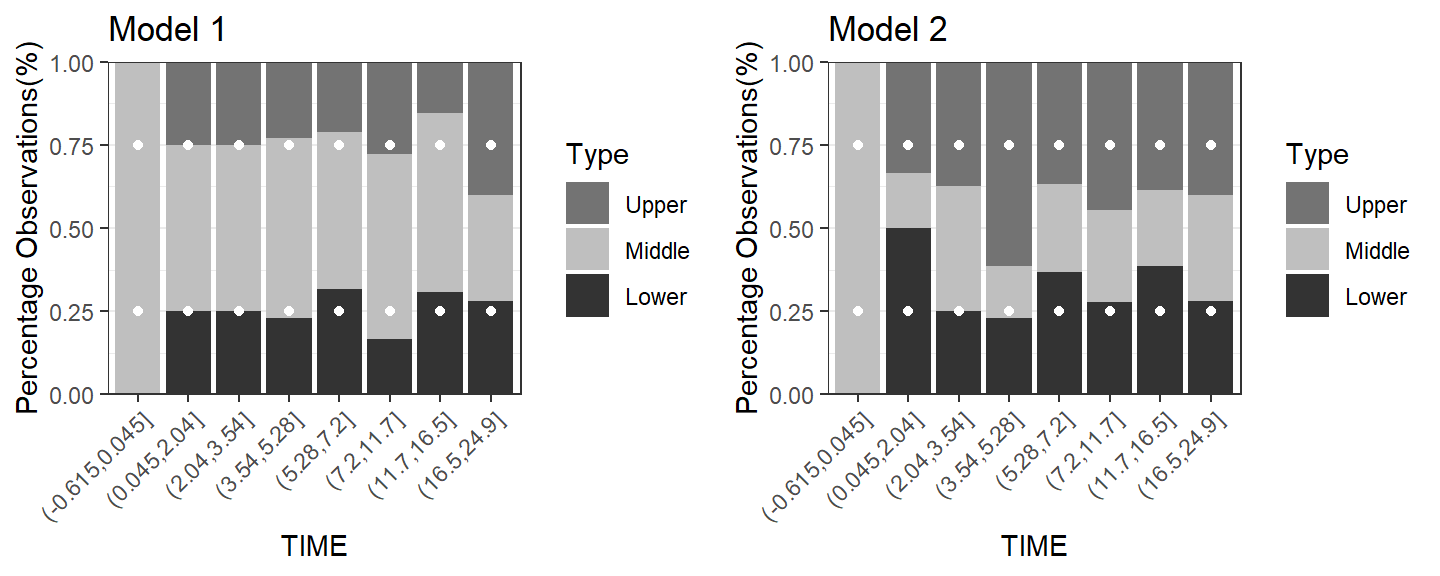
\includegraphics[width=5in,height=2in]{plotPNG/M16-1.png}
\label{M16}
\end{figure}


\begin{figure}
\caption{The coverage detailed plots for Model 1 and Model 2 when PI=80\%.}
\centering
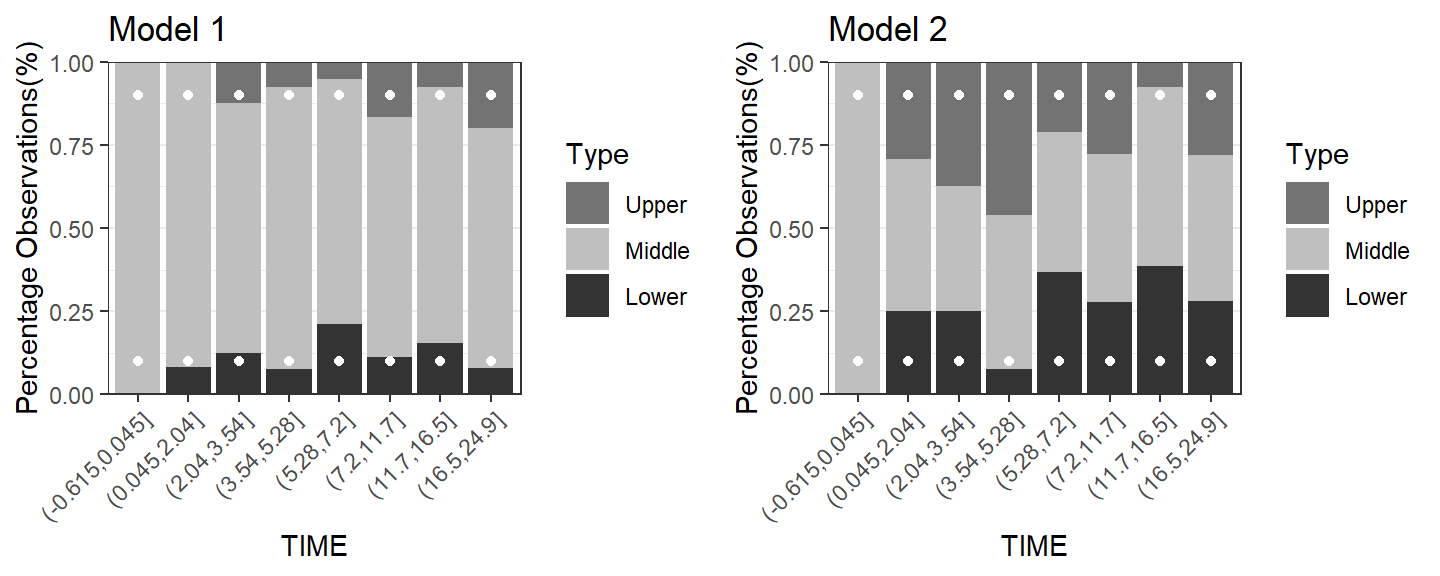
\includegraphics[width=5in,height=2in]{plotPNG/M17-1.png}
\label{M17}
\end{figure}

Figure \ref{M18} shows the results of \code{quantVPC} for Model 1 and Model 2. In Model 2, the right tail area (after 11 hours) looks quite different from the expected pattern. The above percentages are much larger than the below percentages.

The results from Figure \ref{M11} through Figure \ref{M18} show that Model 1 explains the \code{origdata} quite well. However, Model 2 shows different patterns than Model 1 in most figures. We can conclude that Model 1 is better than Model 2, and treating $Ka$ and $Cl$ as random effects is better.

\begin{figure}
\caption{The quantified VPC plots for Model 1 and Model 2.}
\centering
 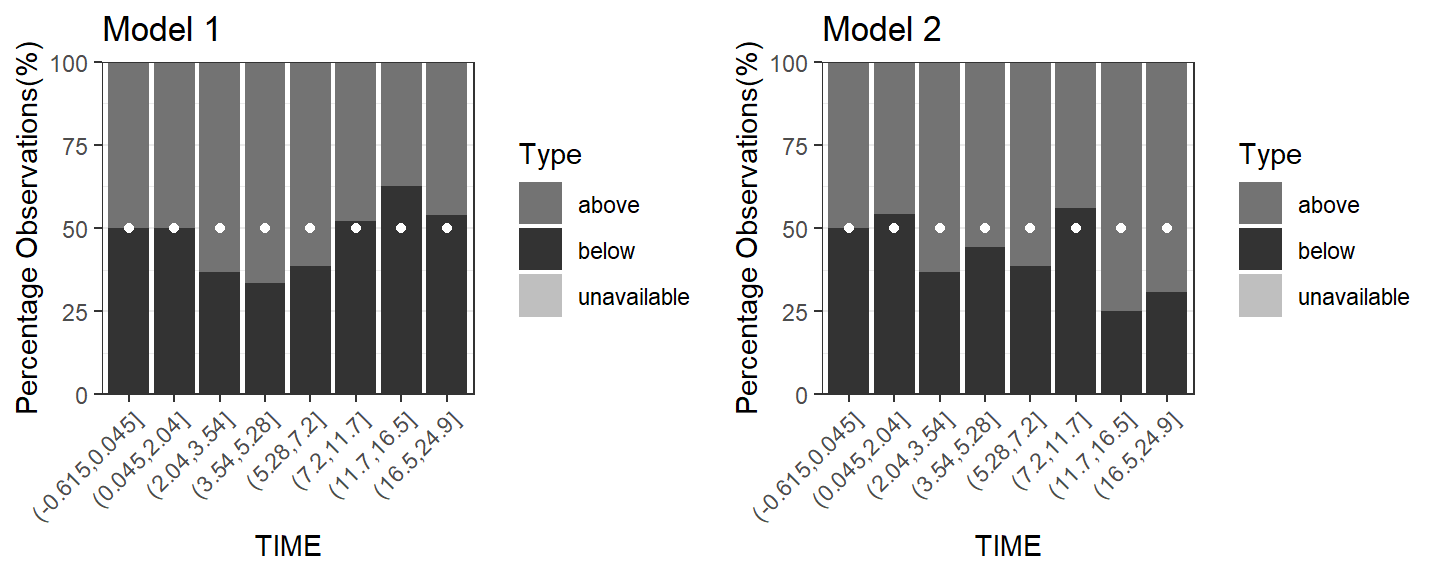
\includegraphics[width=5in,height=2in]{plotPNG/M18-1.png}
\label{M18}
\end{figure}


\hypertarget{Summary}{%
\section{Summary}\label{Summary}}

This paper introduces the \pkg{nlmeVPC} package. The VPC and its extensions are useful for validating the nonlinear mixed effect model. The \pkg{nlmeVPC} package provides various visual diagnostic tools for the nonlinear mixed effect model in two different approaches: validation in data space and model space. Both approaches are valuable. Validation in data space can compare the fitted model with the original data, and validation in model space provides detailed comparisons in various ways. In the \pkg{nlmeVPC} package, we also provide new approaches - \code{asVPC} and \code{coverageDetailplot}. Here, \code{asVPC} provides a more precise VPC plot, and \code{coverageDetailplot} provides the detailed feature of the fitted model that is not captured in the coverage plot. Even though the coverage plot does not show any problem with the fitted model, the coverage detailed plot can reveal the problem in a specific region (Figures \ref{M14}, \ref{M15}, and \ref{M16}).

\hypertarget{Acknowledgements}{%
\section{Acknowledgements}\label{Acknowledgements}}

This work was supported by the National Research Foundation of Korea(NRF) grant funded by the Korea government(MSIT) (2018R1A2B6001251). This paper was prepared by extracting part of Eun-Hwa Kang and Myungji Ko's master thesis.

\bibliography{EunKyung_Lee}

\address{Eun-Hwa Kang\\
  Department of Statistics\\
   Ewha Womans University\\
  Seoul, Korea\\}

\address{Myungji Ko\\
  Department of Statistics\\
   Ewha Womans University\\
  Seoul, Korea\\}

\address{Eun-Kyung Lee\\
  Department of Statistics\\
   Ewha Womans University\\
  Seoul, Korea\\
  (0000-0003-0817-5000)\\
  \email{lee.eunk@ewha.ac.kr}}
